\section{Marco teórico}

\subsubsection{DHT11}

El DHT11 es un sensor digital utilizado para medir temperatura y humedad relativa en aplicaciones de monitoreo ambiental. Integra un sensor capacitivo para la medición de humedad, un termistor tipo NTC para la temperatura y un microcontrolador interno encargado de procesar y enviar los datos mediante una interfaz digital de un solo hilo. Su simplicidad de conexión y bajo costo lo convierten en un dispositivo ampliamente empleado en sistemas educativos, prototipos y proyectos básicos de IoT.

\textbf{Principales características técnicas:}
\begin{itemize}
    \item Alimentación típica entre 3~V y 5.5~V.
    \item Rango de medición de temperatura aproximado entre 0~°C y 50~°C, con resolución de 1~°C.
    \item Rango de medición de humedad relativa entre 20~\% y 90~\%, con resolución de 1~\%.
    \item Comunicación mediante una interfaz digital de un solo bus.
    \item Frecuencia de muestreo típica cercana a 0.5~Hz (una lectura cada dos segundos).
\end{itemize}

Se puede ver el modulo en la figura \ref{}.

\begin{figure}[H]
    \centering
    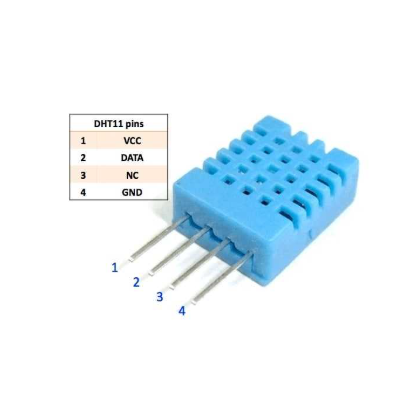
\includegraphics[width=0.3\textwidth]{anexos/1 SPI/DHT11.png}
    \caption{Pulsos DHT11 \url{https://www.alldatasheet.com/html-pdf/2193416/OSEPP/DHT11/1067/6/DHT11.html}}
    \label{fig:S1}
\end{figure}



\subsubsection{Protocolo de Comunicación}

Dicho sensor emplea un protocolo de comunicación digital específico definido por el fabricante como “single‐wire bi–directional serial communication protocol”. Este protocolo propietario se basa en una secuencia de pulsos temporizados en un único hilo de datos. La comunicación comienza cuando el microcontrolador envía una señal de inicio consistente en un pulso bajo prolongado, seguido de un pulso alto de corta duración. Tras esta petición, el DHT11 responde con una secuencia característica de pulsos que indican su disponibilidad y comienza a transmitir los datos.

La información enviada por el sensor se compone de 40 bits organizados en 5 bytes consecutivos: humedad entera, humedad decimal, temperatura entera, temperatura decimal y un byte de verificación (checksum), el cual corresponde a la suma de los cuatro valores anteriores. Cada bit es codificado mediante la duración del pulso alto: un pulso corto representa un ‘0’, mientras que un pulso alto más prolongado representa un ‘1’. Todo el intercambio se realiza por la misma línea de datos. Vease figura \ref{fig:S1} para ver la grafica de pulsos.


\begin{figure}[H]
    \centering
    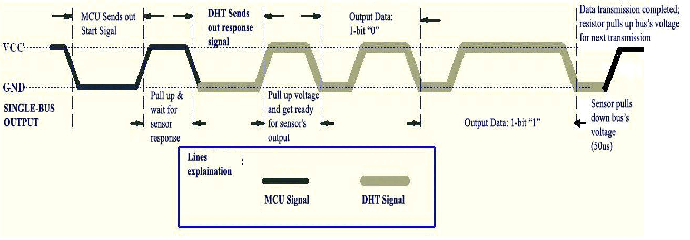
\includegraphics[width=0.3\textwidth]{anexos/1 SPI/Señal DHT1.png}
    \caption{Pulsos DHT11 \url{https://www.alldatasheet.com/html-pdf/2193416/OSEPP/DHT11/1067/6/DHT11.html}}
    \label{fig:S1}
\end{figure}

% Faltan referencias, ya estan hechas , solo nombrarlas

\subsection{Modulo Bluetooth HC05}

El HC-05 es un módulo de comunicación inalámbrica basado en Bluetooth 2.0 diseñado para establecer enlaces serie mediante UART. Permite configurarse tanto en modo maestro como esclavo, lo que facilita la conexión con dispositivos externos como computadoras, teléfonos o microcontroladores. Su simplicidad de uso y compatibilidad con niveles de 3.3~V y 5~V lo convierten en una opción común para proyectos de robótica, domótica y sistemas embebidos que requieren transmisión de datos sin cables.

